%%%%%%%%%%%%%%%%%%%%%%%%%%%%%%%%%%%%%%%%%%%%%%%%%%%%%%%%%%%%%%%%%%%%%%%%%%%%%%%%
\chapter{РАЗРАБОТКА АЛГОРИТМА ИЗВЛЕЧЕНИЯ КОНТРАКТОВ ИЗ ИСХОДНОГО КОДА}
\label{chapter:algoritm}
%%%%%%%%%%%%%%%%%%%%%%%%%%%%%%%%%%%%%%%%%%%%%%%%%%%%%%%%%%%%%%%%%%%%%%%%%%%%%%%%
В соответствии с поставленной задачей, необходимо разработать технологию автоматического извлечения контрактов функций из исходного кода программ. Технология состоит из трех основных этапов:
\begin{itemize}
\item анализ исходного кода программы и выявление предварительных версий контрактов;
\item агрегация полученной информации;
\item построение окончательных версий контрактов для функций из агрегированной  информации;
\end{itemize}

В данном разделе изложены основные идеи, положенные в основу алгоритма. Кроме того рассмотрена модель представления кода????????.

%%%%%%%%%%%%%%%%%%%%%%%%%%%%%%%%%%%%%%%%%%%%%%%%%%%%%%%%%%%%%%%%%%%%%%%%%%%%%%%%
\section{Общая схема алгоритма автоматического извлечения контрактов}
%%%%%%%%%%%%%%%%%%%%%%%%%%%%%%%%%%%%%%%%%%%%%%%%%%%%%%%%%%%%%%%%%%%%%%%%%%%%%%%%
Предлагаемая схема извлечения контрактов из исходного кода в общем виде может быть представлена следующим образом(см. рисунок \ref{image:generalScheme}). На схеме приведен алгоритм извлечения контрактов для одной функции.
\begin{figure}[h!]
\center{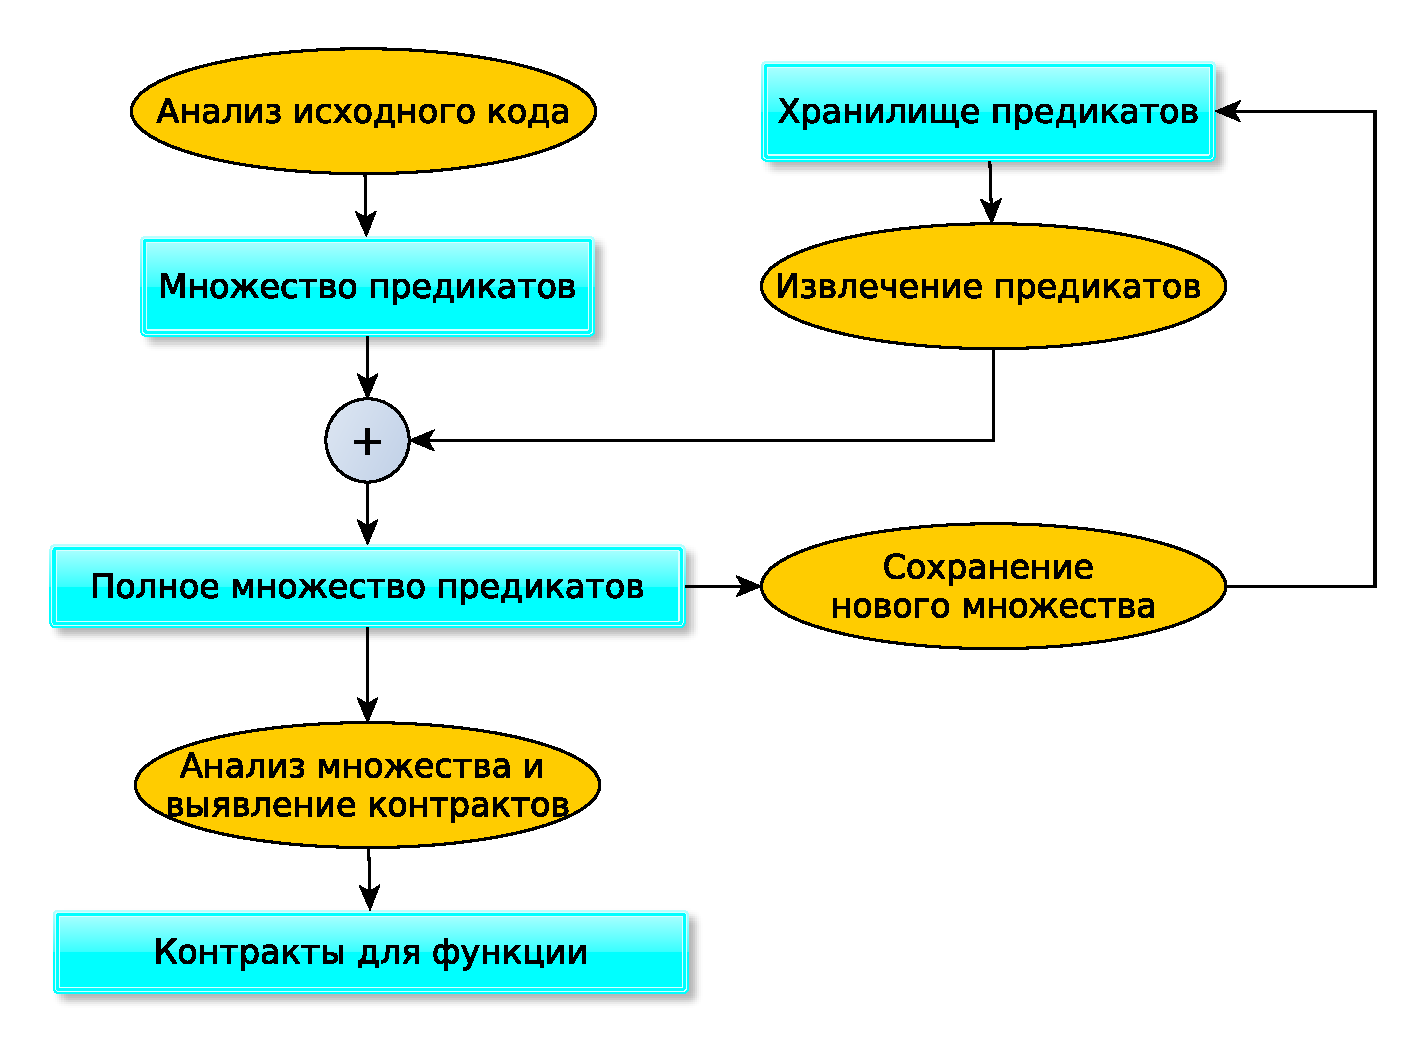
\includegraphics[width=\linewidth]{generalScheme}}
\caption{Общая схема извлечения контрактов из исходного кода}
\label{image:generalScheme}
\end{figure}

Алгоритм принимает на вход исходный код программы. На выходе он возвращает сформированные контракты для функций, используемых в программе. Для повышения эффективности работы алгоритма в нем также используется хранилище предикатов. При выполнении анализа из него извлекается дополнительная информация о функции.

Основным показателем эффективности алгоритма является количество и качество извлекаемых контрактов. Остальные параметры в данной работе считаются второстепенными.

%%%%%%%%%%%%%%%%%%%%%%%%%%%%%%%%%%%%%%%%%%%%%%%%%%%%%%%%%%%%%%%%%%%%%%%%%%%%%%%%
\section{Модель представления кода исходной программы}
%%%%%%%%%%%%%%%%%%%%%%%%%%%%%%%%%%%%%%%%%%%%%%%%%%%%%%%%%%%%%%%%%%%%%%%%%%%%%%%%

%%%%%%%%%%%%%%%%%%%%%%%%%%%%%%%%%%%%%%%%%%%%%%%%%%%%%%%%%%%%%%%%%%%%%%%%%%%%%%%%
\subsection{Система LLVM}
%%%%%%%%%%%%%%%%%%%%%%%%%%%%%%%%%%%%%%%%%%%%%%%%%%%%%%%%%%%%%%%%%%%%%%%%%%%%%%%%
LLVM (Low Level Virtual Machine) --- универсальная система анализа, трансформации и оптимизации программ, реализующая виртуальную машину с RISC-подобными инструкциями. Центральным звеном LLVM является так называемое промежуточное представление (Intermediate Representation, IR), представляющее собой строго типизированный мета-ассемблер с бесконечным числом доступных для использования регистров.  Такая форма представления кода в LLVM (в виде IR) позволяет производить большое количество оптимизаций прямо над промежуточным представлением без необходимости учета особенностей исходного языка программирования, а строгая система типов делает код удобным для восприятия и позволяет производить преобразования, которые не представляется возможным выполнить при обычном трехадресном нетипизированном представлении кода.

Одной из самых важных частей LLVM является система проходов\cite{llvmpass}. Проходы отвечают за трансформацию и оптимизацию промежуточного представления и объединяют результаты различных анализов для их использования в дальнейших преобразованиях.

Программы в LLVM представляются в виде набора отдельных модулей. Каждый модуль состоит из функций, глобальных переменных и дополнительных метаданных. Каждая функция, в свою очередь, состоит из базовых блоков. Каждый базовый блок имеет свою метку и состоит из последовательности инструкций, заканчивающейся инструкцией-терминатором, которая явно передает управление в другой блок или завершает выполнение текущей функции. Пример представления программы в системе LLVM приведен на рисунке \ref{image:llvmIR}.
\begin{figure}[h!]
\center{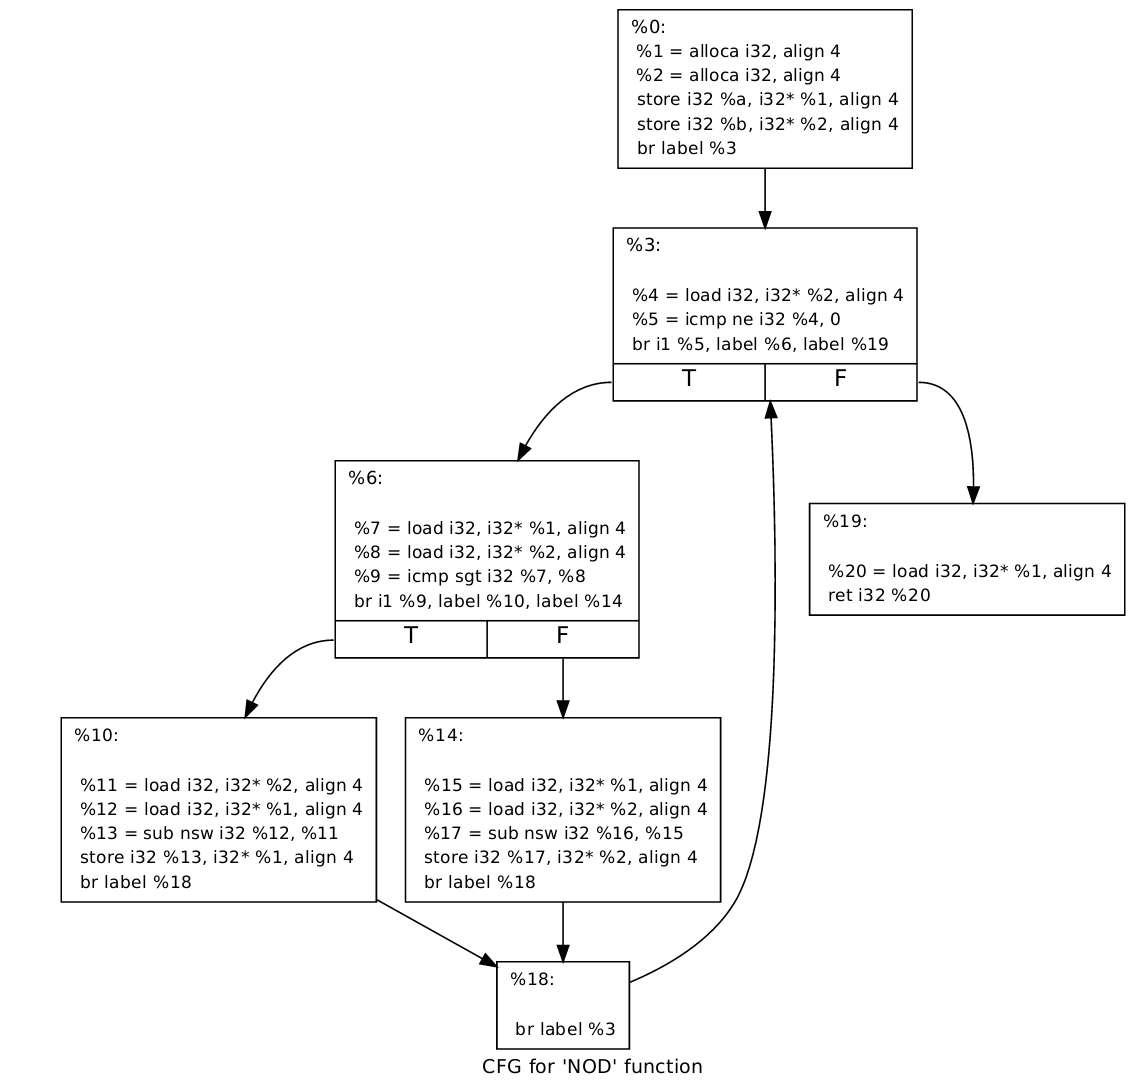
\includegraphics[width=\linewidth]{llvmIR}}
\caption{Пример представления функции в LLVM}
\label{image:llvmIR}
\end{figure}
	
Переменные исходной программы в LLVM представляются в виде регистров (память на стеке) или в виде указателей на память (память на куче). Для регистров LLVM реализует статическое однократное присваивание (Static Single Assigment, SSA) --- форма представления кода, при которой любое значение присваивается только один раз. Любому регистру в LLVM можно присвоить значение только один раз --- при его объявлении. Для объединения потенциально различных значений одной и той же переменной исходной программы в SSA (то есть, и в LLVM) используются так называемые phi-функции, которые возвращают одно из значений в зависимости от того, какой блок передал управление текущему при выполнении программы.

%%%%%%%%%%%%%%%%%%%%%%%%%%%%%%%%%%%%%%%%%%%%%%%%%%%%%%%%%%%%%%%%%%%%%%%%%%%%%%%%
\subsection{Представление программ в системе Borealis}
%%%%%%%%%%%%%%%%%%%%%%%%%%%%%%%%%%%%%%%%%%%%%%%%%%%%%%%%%%%%%%%%%%%%%%%%%%%%%%%%
Система Borealis использует LLVM IR для компиляции, трансформации и анализа программ. Для упрощения взаимодействия различных компонентов Borealis добавляет еще один уровень промежуточного представления в виде Predicate State API (PS API). Упрощенное описание PS приведено на рисунке \ref{image:predicate-state-definition}.
	
Инструкции LLVM преобразуются в предикаты (predicate), которые выполняют различные операции над термами (term). Термы используются для представления констант, переменных, бинарных операций. Каждый терм также может являться операндом другого терма или предиката. Предикаты соответствуют инструкциям LLVM.
	
Предикаты в системе имеют различные типы. Всего определено 6 типов предикатов:
\begin{itemize}
\item State --- обычные предикаты, соответствующие инструкциям LLVM;
\item Path --- предикаты пути соответствуют условиям перехода в различные ветки программы;
\item Requires --- предикаты, использующиеся для выражения предусловий функций;
\item Ensures --- предикаты, использующиеся для выражения постусловий функций;
\item Assert --- предикаты, проверяющиеся на истинность при анализе;
\item Assume --- предикаты, позволяющие задавать утверждения, которые всегда верны.
\end{itemize}

\begin{figure}
	\begin{grammar}
	\scriptsize
	<PredicateState> ::= PredicateStateChain head:<PredicateState> tail:<PredicateState>
	\alt PredicateStateChoice choices:<ListOfPredicateStates>
	\alt BasicPredicateState data:<ListOfPredicates>

	<ListOfPredicateStates> ::= <PredicateState> <ListOfPredicateStates> | <empty>

	<Predicate> ::= AllocaPredicate lhv:<Term> numElems:<Term> origNumElems:<Term>
	\alt DefaultSwitchCasePredicate cond:<Term> cases:<ListOfTerms>
	\alt EqualityPredicate lhv:<Term> rhv:<Term>
	\alt GlobalsPredicate globals:<ListOfTerms>
	\alt InequalityPredicate lhv:<Term> rhv:<Term>
	\alt MallocPredicate lhv:<Term> numElems:<Term> origNumElems:<Term>
	\alt SeqDataPredicate base:<Term> data:<ListOfTerms>
	\alt SeqDataZeroPredicate base:<Term> size:UInt32
	\alt StorePredicate ptr:<Term> value:<Term>
	\alt WriteBoundPredicate ptr:<Term> boundValue:<Term>
	\alt WritePropertyPredicate propName:<Term> ptr:<Term> propValue:<Term>
	
	\tiny
	<Term> ::= ArgumentTerm idx:UInt32 kind:<ArgumentKind>
	\alt ArgumentCountTerm
	\alt AxiomTerm term:<Term> axiom:<Term>
	\alt BinaryTerm op:<BinaryOp> lhv:<Term> rhv:<Term>
	\alt BoundTerm term:<Term>
	\alt CastTerm term:<Term> signExtend:Bool
	\alt CmpTerm op:<CmpOp> lhv:<Term> rhv:<Term>
	\alt ConstTerm
	\alt FreeVarTerm
	\alt GepTerm base:<Term> shifts:<ListOfTerms> triviallyInbounds:Bool
	\alt LoadTerm ptr:<Term>
	\alt OpaqueBigIntConstantTerm value:String
	\alt OpaqueBoolConstantTerm value:Bool
	\alt OpaqueBuiltinTerm vname:String
	\alt OpaqueCallTerm func:<Term> args:<ListOfTerms>
	\alt OpaqueFloatingConstantTerm value:Double
	\alt OpaqueIndexingTerm value:<Term> index:<Term>
	\alt OpaqueIntConstantTerm value:SInt64
	\alt OpaqueInvalidPtrTerm
	\alt OpaqueMemberAccessTerm value:<Term> property:String indirect:Bool
	\alt OpaqueNamedConstantTerm vname:String
	\alt OpaqueNullPtrTerm 
	\alt OpaqueStringConstantTerm value:String
	\alt OpaqueUndefTerm 
	\alt OpaqueVarTerm vname:String
	\alt ReadPropertyTerm propName:<Term> ptr:<Term>
	\alt ReturnPtrTerm funcName:String
	\alt ReturnValueTerm funcName:String
	\alt SignTerm value:<Term>
	\alt TernaryTerm cond:<Term> tru:<Term> fls:<Term>
	\alt UnaryTerm op:<UnaryOp> value:<Term>
	\alt ValueTerm global:Bool
	\alt VarArgumentTerm index:UInt32

	<ListOfTerms> ::= <Term> <ListOfTerms> | <empty>

	<ArgumentKind> ::= ANY | STRING

	<BinaryOp> ::= ...
	<UnaryOp> ::= ...
	<CmpOp> ::= ...
	\end{grammar}
	
\caption{Определение предикатного состояния}
\label{image:predicate-state-definition}
\end{figure}

Predicate state ставится в соответствие каждой функции программы. При этом, как показано на рисунке \ref{image:predicate-state-definition}, PS может состоять как из предикатов, так и из других predicate state'ов. Вложенные PS обычно соответствуют базовым блокам LLVM IR. Predicate state бывает трех видов:
\begin{enumerate}
\item Basic PS --- PS, соответствующий базовым блокам LLVM.
\item Choice PS --- PS, который позволяет реализовывать ветвления. Каждой веткой choice PS выбора может быть любой другой PS. Это позволяет представлять операторы множественного выбора и множественные ветвления. При этом стоит отметить, что в начале каждого PS, соответствующего какой-либо ветке, будет стоять path predicate, определяющий условия входа в эту ветку.
\item Chain PS --- PS, позволяющий объединить несколько PS в единую последовательность. Используется для соединения Basic PS и Choice PS в единую структуру, аналогичную графу потока управления исходной программы.
\end{enumerate}

%%%%%%%%%%%%%%%%%%%%%%%%%%%%%%%%%%%%%%%%%%%%%%%%%%%%%%%%%%%%%%%%%%%%%%%%%%%%%%%%
\subsection{Использование SMT решателей для анализа программ}
%%%%%%%%%%%%%%%%%%%%%%%%%%%%%%%%%%%%%%%%%%%%%%%%%%%%%%%%%%%%%%%%%%%%%%%%%%%%%%%%
SMT (satisfiability modulo theories) --- это задача разрешимости для логических формул с учетом лежащих в их основе теорий\cite{smt}. SMT решатели --- инструменты для решения SMT задач. Идея использования SMT решателей для анализа программ состоит в том, чтобы преобразовать исходную программу в SMT формулу и проверить ее на выполнимость (satisfiability). Для упрощения взаимодействия с различными SMT решателями Borealis использует PS. На данный момент Borealis поддерживает два разных SMT решателя: MathSAT\cite{mathsatsolver} и Z3. Для преобразования PS в SMT необходимо определить правила трансляции. Преобразование большинства термов и предикатов достаточно очевидно: TernaryTerm выбирает одно из двух значений в зависимости от третьего, GepTerm соответствует LLVM инструкции GetElementPointer и т.д. Переменные программы представляются в виде битовых векторов соответствующей размерности. Проблемой являются инструкции работы с памятью, так как память не так просто выразить в терминах SMT.

Borealis использует подход, схожий с LLBMC\cite{llbmc}. Память представляется как массив??????? с определенными операциями записи (StorePredicate) и чтения (LoadTerm)\cite{smtlib}.

Предлагаемый подход автоматического извлечения контрактов будет описываться в терминах приведенной модели кода. Перейдем к более подробному рассмотрению этапов предлагаемой методологии.

%%%%%%%%%%%%%%%%%%%%%%%%%%%%%%%%%%%%%%%%%%%%%%%%%%%%%%%%%%%%%%%%%%%%%%%%%%%%%%%%
\section{Анализ исходного кода программы для извлечения предварительных версий контрактов}
\label{section:analysis}
%%%%%%%%%%%%%%%%%%%%%%%%%%%%%%%%%%%%%%%%%%%%%%%%%%%%%%%%%%%%%%%%%%%%%%%%%%%%%%%%
Все статические подходы автоматического извлечения контрактов сталкиваются с необходимостью анализа исходного кода. Для извлечения контрактов необходимо сперва определить, в каких участках исходного кода (или, может быть, каких-либо сопутствующих артефактов) следует искать возможные контракты. Различные подходы по своему решают эту проблему.

В данной работе предлагается анализировать места вызова функций с целью определения условных операторов, в которых каким-либо образом используются аргументы, передаваемые в эту функцию. Определяя подобным образом условные операторы, предшествующие вызову функции, можно извлекать предусловия для этих функций.

Предлагаемый алгоритм извлечения предварительного множества предусловий выглядит следующим образом:
\begin{enumerate}
\item редукция предикатов равенства;
\item определение всех условий, использующих аргументы функции;
\item отбрасывание заведомо неверных условий.
\end{enumerate}

Рассмотрим каждый пункт алгоритма более подробно.

%%%%%%%%%%%%%%%%%%%%%%%%%%%%%%%%%%%%%%%%%%%%%%%%%%%%%%%%%%%%%%%%%%%%%%%%%%%%%%%%
\subsection{Редукция предикатов равенства}
\label{subsection:reduction}
%%%%%%%%%%%%%%%%%%%%%%%%%%%%%%%%%%%%%%%%%%%%%%%%%%%%%%%%%%%%%%%%%%%%%%%%%%%%%%%%
В системе LLVM используется SSA. Каждой переменной исходного кода в ассемблере LLVM может соответствовать несколько регистров. Особенно остро эта проблема проявляется для переменных, расположенных  в памяти. При каждом использовании подобной переменной будет создан новый регистр. Это усложняет анализ программы в LLVM, так как появляется необходимость отслеживания зависимостей между переменными.

Для решения данной проблемы используется редукция предикатов равенства: переменные в правой части предикатов равенства заменяются на их определения. Эта операция позволяет значительно упростить следующие этапы алгоритма. Пример выполнения подобной операции приведен на рисунке \ref{image:equalityMapperExample}.
\begin{figure}[h!]
\center{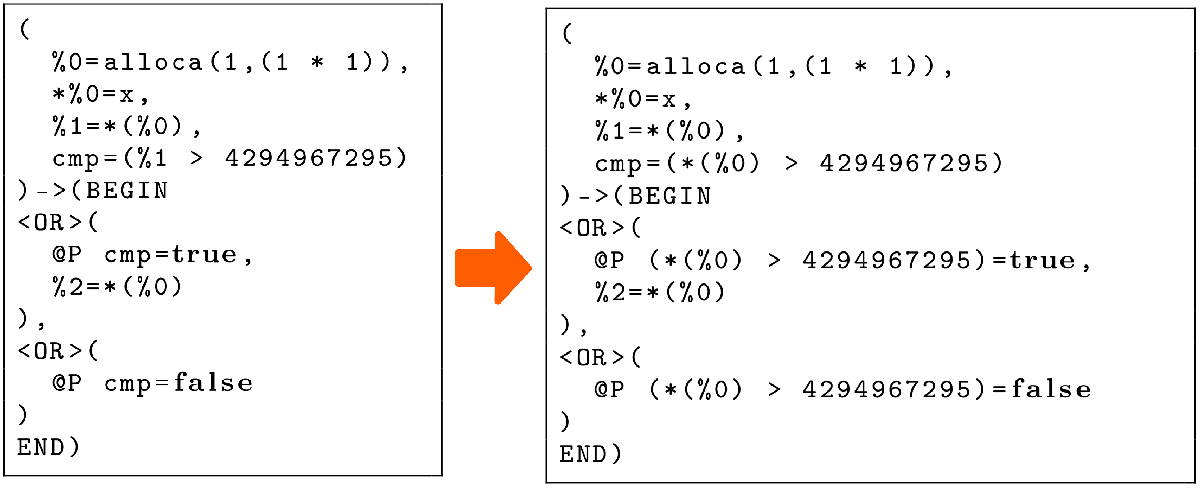
\includegraphics[width=\linewidth]{equalityMapperExample}}
\caption{Пример редукции предикатов равенства}
\label{image:equalityMapperExample}
\end{figure}

%%%%%%%%%%%%%%%%%%%%%%%%%%%%%%%%%%%%%%%%%%%%%%%%%%%%%%%%%%%%%%%%%%%%%%%%%%%%%%%%
\subsection{Алгоритм извлечения предварительного множества предусловий}
\label{subsection:extraction}
%%%%%%%%%%%%%%%%%%%%%%%%%%%%%%%%%%%%%%%%%%%%%%%%%%%%%%%%%%%%%%%%%%%%%%%%%%%%%%%%
Как было отмечено ранее, в данной работе предлагается анализировать места вызова функций с целью определения условных операторов, в которых каким-либо образом используются аргументы, передаваемые в эту функцию. Определенные подобным образом предикаты являются предусловиями в двух случаях:
\begin{itemize}
\item если в одной из веток условного оператора происходит выход из функции;
\item если вызов функции происходит внутри блока условного оператора.
\end{itemize}

В принятой модели представления кода первый случай объединяется со вторым, так как система Borealis автоматически приводит все условные операторы к необходимому виду. Это происходит благодаря тому, что в функции в Borealis может быть только один оператор <<return>> (пример приведен на рисунке \ref{image:llvmIFcfg}).
\lstinputlisting[
label={listing:llvmIFexample},
caption={Пример функции на языке С},
]{src/llvmIFexample.c}
 	
\begin{figure}[h!]
\center{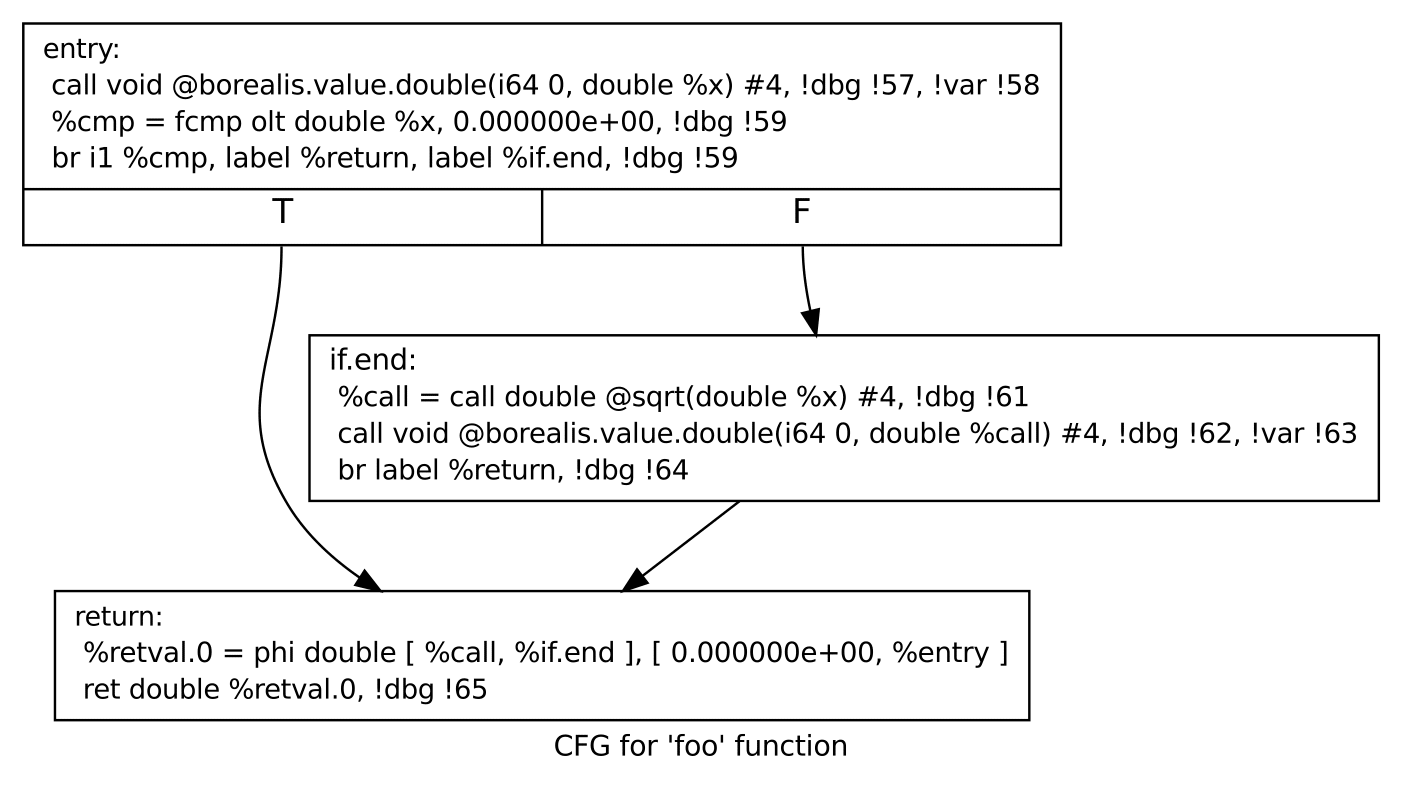
\includegraphics[width=\linewidth]{llvmIFcfg}}
\caption{Представление функции из листинга \ref{listing:llvmIFexample} в LLVM IR после преобразований, выполняемых в Borealis'е}
\label{image:llvmIFcfg}
\end{figure}

В системе Borealis функция из листинга \ref{listing:llvmIFexample} будет представлена в следующем виде (см. листинг \ref{listing:llvmIFexampleBorealis}). Вызов функции sqrt() отсутствует в этом представлении, так как система Borealis поддерживает межпроцедурный анализ только для функций, для которых определена какая-либо дополнительная информация (контракты, аппроксимации, аннотации).
\lstinputlisting[
label={listing:llvmIFexampleBorealis},
caption={Представление функции из листинга \ref{listing:llvmIFexample} в Borealis},
]{src/llvmIFexampleBorealis}

При анализе PS функции рассматривается относительно точки вызова функции. Соответственно, если условный оператор удовлетворяет поставленным требованиям (то есть вызов функции происходит внутри блока этого условного оператора), в PS будет представлена только одна ветка условного оператора (та, в которой происходит вызов функции). Если вызов функции происходит вне блока условного оператора, то в результирующем PS будут представлены обе ветки условного оператора.

Согласно представлению Borealis, в начале каждой ветки программы присутствуют предикаты пути (path predicates), которые определяют условия входа в эту ветку. Соответственно, при анализе программы необходимо извлекать предикаты пути, которые предшествуют вызовам функции. Если предикаты пути образуют полную группу событий, значит вызов функции происходит вне блока условного оператора. В результате анализа исходного кода извлекается множество предикатов, из которого далее можно выявить предусловия функции.

%%%%%%%%%%%%%%%%%%%%%%%%%%%%%%%%%%%%%%%%%%%%%%%%%%%%%%%%%%%%%%%%%%%%%%%%%%%%%%%%
\section{Хранение результатов анализа}
\label{section:saving}
%%%%%%%%%%%%%%%%%%%%%%%%%%%%%%%%%%%%%%%%%%%%%%%%%%%%%%%%%%%%%%%%%%%%%%%%%%%%%%%%
Для увеличения точности работы алгоритма предлагается сохранять все найденные множества предикатов в базу данных для их последующего использования при формировании контрактов. Это позволит уменьшить вероятность некорректного извлечения контракта, так как увеличится множество предикатов, из которого в последующем будет извлекаться контракт. Кроме того, это позволит формировать контракты для тех функций, для которых не было получено никакой информации из исходного кода текущей программы.

В предлагаемом подходе для каждой функции сохраняются:
\begin{itemize}
\item уникальный идентификатор функции;
\item количество встреченных вызовов функции;
\item полученное в результате анализа множество предикатов.
\end{itemize}

Уникальный идентификатор функции используется в качестве ключа в базе данных. Идентификатор должен позволять точно идентифицировать функцию и получать для нее необходимую информацию из базы. В данной работе было принято, что для идентификации функции достаточно хранить ее имя и тип возвращаемого значения. Вероятность ошибочно сопоставить две разные функции как одну при этом ниже, чем при хранении только имени функции. Однако, эта вероятность не равна нулю. Возможны случаи, когда будут найдены две функции с одинаковым именем и типом возвращаемого значения, но с разными аргументами. К тому же, даже если функции будут иметь одинаковую сигнатуру, они могут иметь различную реализацию.

%%%%%%%%%%%%%%%%%%%%%%%%%%%%%%%%%%%%%%%%%%%%%%%%%%%%%%%%%%%%%%%%%%%%%%%%%%%%%%%%
\section{Формирование предусловий для функции}
\label{section:merging}
%%%%%%%%%%%%%%%%%%%%%%%%%%%%%%%%%%%%%%%%%%%%%%%%%%%%%%%%%%%%%%%%%%%%%%%%%%%%%%%%
Целью данного этапа является формирование окончательных версий предусловий для функции из полученного ранее множества предикатов. Основная идея: предусловиями функции являются предикаты, которые достаточно часто встречаются в местах ее вызова. 

Для повышения скорости работы алгоритма первым шагом из исходного множества предикатов $P$ выделяется множество уникальных предикатов $P'$ и для каждого уникального предиката $P'_i$ определяется $N_i$ --- сколько раз данный предикат встречался в исходном множестве. Все последующие операции будут производиться над множеством $P'$.

На данном этапе необходимо решить несколько задач:
\begin{itemize}
\item определить что делать с предикатами, условия которых противоположны друг-другу;
\item определить правила слияния <<схожих>> предикатов, то есть предикатов, условия которых каким-либо образом пересекаются;
\item определить насколько часто должен встречаться предикат, чтобы его можно было использовать в качестве предусловия.
\end{itemize}

%%%%%%%%%%%%%%%%%%%%%%%%%%%%%%%%%%%%%%%%%%%%%%%%%%%%%%%%%%%%%%%%%%%%%%%%%%%%%%%%
\subsection{Алгоритм удаления противоположных условий}
%%%%%%%%%%%%%%%%%%%%%%%%%%%%%%%%%%%%%%%%%%%%%%%%%%%%%%%%%%%%%%%%%%%%%%%%%%%%%%%%
В исходном коде перед вызовом функции в разных местах могут встречаться предикаты с противоположными условиями.\footnote{Здесь и далее термины <<предикат>> и <<условие>> используются как синонимы, так как предикаты пути, над которыми выполняются операции, являются условиями выполнения этого пути.} Выявление противоположных условий выполняется с помощью SMT решателя. 

Предикаты с противоположными условиями могут встречаться в двух случаях:
\begin{itemize}
\item в исходном коде имеется ошибка и один из найденных предикатов является некорректным;
\item найденные предикаты никак не влияют на поведение функции и не являются предусловиями.
\end{itemize}
Детектирование первого случая может улучшить результаты работы алгоритма (и, соответственно, статического анализа). Однако в общем случае невозможно определить разницу между первым и вторым случаем. Было решено удалять предикаты с противоположными условиями из множества $P'$ (при этом соответствующие данным предикатам элементы множества $N'$ так же удаляются), так как главной целью разработки методологии является ее безопасность.

%%%%%%%%%%%%%%%%%%%%%%%%%%%%%%%%%%%%%%%%%%%%%%%%%%%%%%%%%%%%%%%%%%%%%%%%%%%%%%%%
\subsection{Алгоритм слияния множества предикатов}
%%%%%%%%%%%%%%%%%%%%%%%%%%%%%%%%%%%%%%%%%%%%%%%%%%%%%%%%%%%%%%%%%%%%%%%%%%%%%%%%
Следующим шагом является слияние схожих предикатов. Схожими  считаются предикаты, условия которых каким-либо образом пересекаются. Для этого в множестве $P'$ необходимо оставить только подмножество $P^*$, которое содержит в себе слабейшие условия из множества $P'$. Решение использовать слабейшие условия связано с тем, что они накладывают наименьшие возможные ограничения на аргументы функции, соответственно вероятность извлечения неверного предусловия так же уменьшается. При этом так же необходимо сформировать множество $N^*$, которое содержит информацию о том, сколько раз условие каждого предиката из множества $P^*$ выполнялось перед вызовом функции. Алгоритм построения подмножества $P^*$ приведен ниже (см. рисунок \ref{image:megringAlgoritm}). Функция $isWeaker(p_1, p_2)$, использованная в этом алгоритме, возвращает истинное значение, если условие $p_1$ слабее условия $p_2$. Соответственно, каждую пару предикатов необходимо проверить два раза: слабее ли $p_1$ чем $p_2$ и наоборот. Сравнение предикатов в этой функции выполняется с помощью SMT решателя. Для этого исполь­зуется операция импликации: в SMT решатель подается форму­ла $\overline{p_2 \Longrightarrow p_1}$. Если формула невыполнима, значит первый предикат слабее второго.
\begin{figure}[h!]
\textbf{Вход:} $P'$ --- множество уникальных предикатов

\textbf{Вход:} $N'$ --- сколько раз каждый предикат из $P'$ встречался перед вызовом функции

\textbf{Выход:} $P^*$ --- множество слабейших предикатов

\textbf{Выход:} $N^*$ --- сколько раз условие каждого предиката из $P^*$ выполнялось перед вызовом функции

\begin{algorithmic}[1]
\State $P'' \leftarrow \emptyset$
\State $N'\ \leftarrow \emptyset$
\ForAll {$p_i \in P'$}
	\ForAll {$p_j \in P'$}
		\If {$isWeaker(p_i, p_j)$}
			\State $P' \leftarrow P' \backslash P'_j$;
			\State $N'_i = (N'_i + N'_j)$;
			\State $N' \leftarrow N' \backslash N'_j$;
		\Else 
			\If {$isWeaker(p_j, p_i)$}
				\State $P' \leftarrow P' \backslash P'_i$;
				\State $N'_j = (N'_i + N'_j)$;
				\State $N' \leftarrow N \backslash N'_i$;
    			\EndIf
    		\EndIf
    \EndFor
\EndFor
\State $P^* \leftarrow P'$
\State $N^* \leftarrow N'$
\end{algorithmic}
\caption{Алгоритм слияния предикатов}
\label{image:megringAlgoritm}
\end{figure}

%%%%%%%%%%%%%%%%%%%%%%%%%%%%%%%%%%%%%%%%%%%%%%%%%%%%%%%%%%%%%%%%%%%%%%%%%%%%%%%%
\subsection{Алгоритм формирования предусловий}
%%%%%%%%%%%%%%%%%%%%%%%%%%%%%%%%%%%%%%%%%%%%%%%%%%%%%%%%%%%%%%%%%%%%%%%%%%%%%%%%
Последним этапом технологии является формирование множества предусловий $C$ для функции. Множество выявляется на основе анализа частоты появления предикатов перед вызовом функции. Предлагаемый
алгоритм приведен ниже (см. рисунок \ref{image:extractionAlgoritm}).
\begin{figure}[h!]
\textbf{Вход:} $K$ --- константа слияния $0 \le K \le 1$

\textbf{Вход:} $X$ --- минимальное число вызовов функции $X \ge 0$

\textbf{Вход:} $P^*$ --- множество слабейших предикатов

\textbf{Вход:} $N^*$ --- сколько раз условие каждого предиката из $P^*$ выполнялось перед вызовом функции

\textbf{Вход:} $M$ --- число вызовов функции

\textbf{Выход:} $C$ --- множество предусловий
\begin{algorithmic}[1]
\State $C \leftarrow \emptyset$
\If {$M < X$}
	\State \Return
\EndIf
\ForAll {$p_i \in P''$}
	\If {${N'[i]}/{M} \leq K$;}
	\State $C \gets C \cup p_i$;
    \EndIf
\EndFor
\end{algorithmic}
\caption{Алгоритм формирования предусловий}
\label{image:extractionAlgoritm}
\end{figure}

Качество работы данного алгоритма во многом определяется константами $K$ и $X$, от которых зависит полнота и точность анализа. Константа $K$ определяет как часто предикат должен встречаться в точках вызова функции для того, чтобы его можно было считать предусловием. При $K \to 1$ повышается точность алгоритма, но понижается его полнота. Кроме того, при $K \to 1$ полученные предусловия окажут минимальное влияние на результаты анализа (так как найденные контракты и без этого будут выполняться в большинстве случаев вызова функций). При $K \leftarrow 0$ повышается полнота анализа, но понижается точность. При низкой точности анализа повышается вероятность извлечения ошибочного контракта. 

Константа $X$ определяет минимальное число вызовов функции, при котором алгоритм может делать какие-то выводы о ее поведении. При $X \to 0$ полнота алгоритма максимальна, однако  понижается точность алгоритма. При $X \to \infty$ вероятность ошибки стремится к 0, однако понижается полнота. Для получения качественных результатов необходимо найти компромисс между двумя этими свойствами.

\section{Резюме}
В данном разделе представлена технология автоматического извлечения контрактов функций, основанная на статическом анализе исходного кода программ. Рассмотрена модель представления кода, используемая в данной технологии. Описаны основные компоненты технологии, такие как: алгоритм анализа исходного кода для выявления предварительного множества предикатов, способ хранения результатов анализа, алгоритм формирования предусловий для функции на основе результатов анализа.